\chapter{Implementacja systemu}
\label{c:implementacja}

\section{Wykorzystane technologie i organizacja projektu}

Implementacja systemu obejmuje część mobilną, serwerową oraz narzędzia pomocnicze do przygotowywania danych i uczenia modeli. Podział ten odpowiada założonej architekturze klient--serwer przedstawionej w rozdziale \ref{c:koncepcja}.

Do przygotowania aplikacji mobilnej wykorzystano technologię Kotlin Multiplatform oraz Compose Multiplatform. Ich użycie umożliwiło stworzenie pojedynczej bazy kodu możliwej do uruchomienia zarówno na systemie Android, jak i iOS, przy jednoczesnym zachowaniu osobnych implementacji elementów zależnych od platformy. Aplikacja implementuje funkcjonalności transmisji obrazu, komunikacji z serwerem, interfejs użytkownika oraz zarządzania stanem. Komunikacja jest realizowana za pomocą biblioteki \texttt{Ktor}.

Część serwerowa została zaimplementowana w języku Python. Do obsługi połączenia sieciowego wykorzystano bibliotekę \texttt{websockets}, a do dekodowania obrazu i jego przetwarzania bibliotekę \texttt{OpenCV}. Inferencja modeli sieci neuronowych odbywa się przy użyciu biblioteki \texttt{Ultralytics}, która działa w środowisku \texttt{PyTorch}. Interfejs graficzny przygotowano przy użyciu biblioteki \texttt{PySide6}.

Najważniejsze technologie wykorzystane w implementacji poszczególnych komponentów systemu zostały zestawione w tabeli \ref{tab:technologie_systemu}.

Repozytorium rozwiązania składa się z pięciu katalogów:

\begin{itemize}
    \item \texttt{KMP} -- aplikacja mobilna dla systemów Android i iOS;
    \item \texttt{server} -- część serwerowa systemu;
    \item \texttt{training} -- katalog narzędzi do trenowania modeli sieci neuronowych;
    \item \texttt{dataset\_splitter} -- skrypt do podziału zbioru danych;
    \item \texttt{video\_to\_dataset} -- narzędzie do ekstrakcji klatek z nagrań wideo.
\end{itemize}

Rozdzielenie kodu poszczególnych części umożliwia niezależny rozwój i testowanie komponentów systemu. Szczególnie istotne jest rozdzielenie narzędzi związanych z przygotowaniem danych i trenowaniem modeli od kodu aplikacji mobilnej i serwera. Wyznacza to wyraźne granice między częścią wykonawczą systemu i jego komponentami badawczymi.

\begin{table}[htbp]
    \centering
    \caption{Najważniejsze technologie wykorzystane w poszczególnych częściach systemu}
    \label{tab:technologie_systemu}
    \begin{tabularx}{\textwidth}{
        l >{\raggedright}p{5cm} X
        }
        \toprule

        \textbf{Część systemu}                               & \textbf{Technologie i biblioteki} & \textbf{Zastosowanie} \\

        \midrule

        Aplikacja\newline mobilna                            &
        Kotlin Multiplatform, Compose Multiplatform, Ktor    &
        Współdzielona logika aplikacji, interfejs użytkownika i komunikacja \nolinebreak{WebSocket}                      \\

        \addlinespace

        Android                                              &
        CameraX, SpeechRecognizer, TextToSpeech, Android NSD &
        Rejestrowanie obrazu, rozpoznawanie komend głosowych, synteza mowy i wykrywanie serwera w sieci lokalnej         \\

        \addlinespace

        iOS                                                  &
        AVFoundation, SwiftUI                                &
        Rejestrowanie obrazu, podgląd kamery i osadzenie współdzielonego interfejsu aplikacji                            \\

        \addlinespace

        Część serwerowa                                      &
        Python, websockets, OpenCV, Ultralytics, PyTorch, webcolors     &
        Obsługa komunikacji, dekodowanie i przetwarzanie obrazu, wykonywanie detekcji obiektów i dopasowanie kolorów powierzchni                                          \\

        \addlinespace

        Interfejs serwera                                    &
        PySide6, QWebChannel                                 &
        Prezentowanie obrazu, stanu połączenia i bieżących wyników detekcji                                              \\

        \addlinespace

        Narzędzia\newline badawcze                           &
        Ultralytics, OpenCV, NumPy, scikit-learn, matplotlib &
        Przygotowanie zbioru danych, uczenie, testowanie i analiza wyników modeli                                        \\

        \bottomrule
    \end{tabularx}
\end{table}

\section{Implementacja aplikacji mobilnej}
\label{s:implementacja_aplikacji}

Aplikacja mobilna stanowi część kliencką systemu. Do jej zadań należy rejestrowanie obrazu z kamery urządzenia, przekazywanie kolejnych klatek do serwera, oraz obsługa bezdotykowa systemu za pomocą komend głosowych. Podział aplikacji przedstawiono na diagramie komponentów, na rysunku \ref{fig:diagram_komponentow_aplikacji}.

\clearpage
\begin{sidewaysfigure}[p]
    \centering

    \begin{center}
        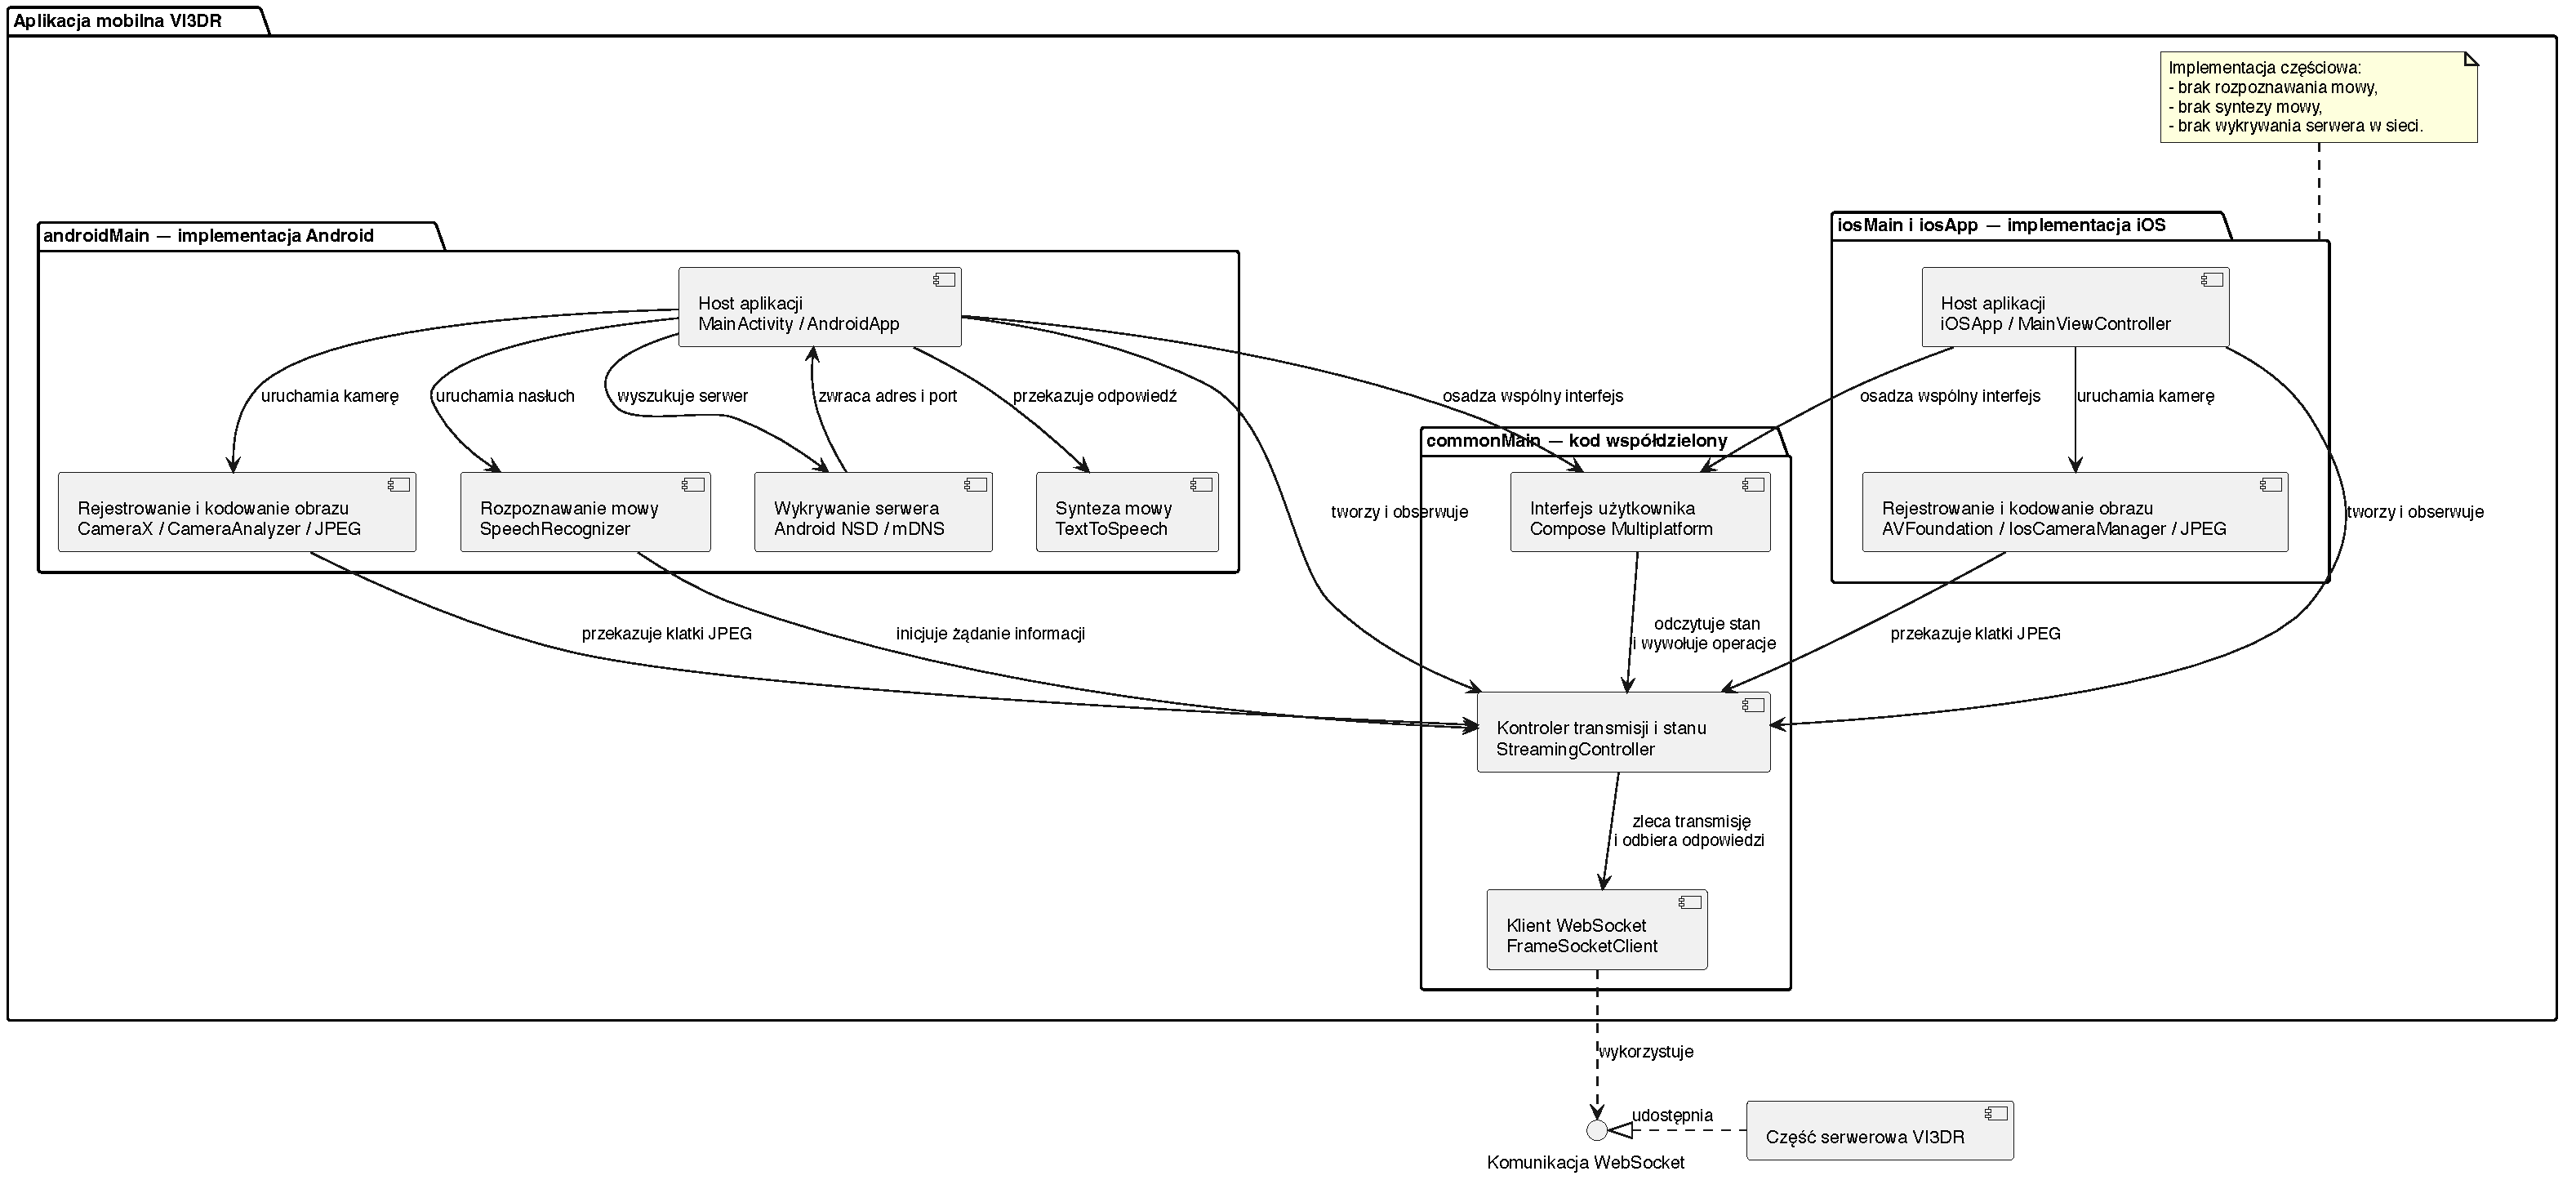
\includegraphics[
            width=\textheight,
            height=\linewidth,
            keepaspectratio]
            {./graf/diagram_mobilka.pdf}

        \captionof{figure}{Diagram komponentów aplikacji mobilnej z podziałem na kod współdzielony i implementacje platformowe}
        \label{fig:diagram_komponentow_aplikacji}
    \end{center}
    
\end{sidewaysfigure}

\clearpage

\subsection{Organizacja kodu aplikacji}

Implementacja aplikacji mobilnej została zrealizowana z wykorzystaniem technologii Kotlin Multiplatform i Compose Multiplatform. Kod aplikacji umieszczono w module \texttt{composeApp} i podzielono na pakiety odpowiadające częściom wspólnym i zależnym od platformy. W katalogu \texttt{commonMain} znajduje się kod współdzielony obsługujący logikę zarządzania stanem aplikacji, komunikację z serwerem, obsługę połączenia oraz wspólne elementy interfejsu użytkownika. Katalogi \texttt{androidMain} i \texttt{iosMain} zawierają implementacje korzystające z natywnych funkcji systemów Android i iOS, takich jak rejestrowanie obrazu, obsługa komend głosowych i odczytywanie komunikatów z serwera.

Centralny punkt aplikacji stanowi klasa \texttt{StreamingController}, zarządzająca stanem połączenia i transmisji. Kontroluje ona również częstotliwość przesyłania kolejnych klatek oraz obsługuje żądania użytkownika i odpowiedzi serwera. Stan kontrolera wykorzystywany jest przez interfejs użytkownika przygotowany w technologii Compose Multiplatform. Do współdzielonego interfejsu użytkownika dołączany jest natywny podgląd z kamery urządzenia.

Zastosowanie technologii Kotlin Multiplatform umożliwiło rozpoczęcie prac nad aplikacją mobilną jednocześnie dla systemów Android i iOS. Wstępne testy implementacji ukazały jednak istotne problemy ze stabilnością i wydajnością aplikacji na systemie iOS. Z tego względu dalsze prace skupiono wyłącznie na aplikacji dla systemu Android, dla której zaimplementowano wszystkie funkcjonalności systemu. Kod aplikacji dla systemu iOS pozostawiono w repozytorium aby umożliwić dalszy rozwój tej gałęzi w przyszłości.

\subsection{Rejestrowanie i przygotowanie obrazu}

Punktem wejścia do aplikacji jest klasa \texttt{MainActivity}, która uruchamia interfejs użytkownika i konfiguruje elementy wymagające dostępu do natywnych mechanizmów systemu: kamery, mikrofonu i syntezatora mowy. Rejestrowanie obrazu z kamery realizowane jest przy użyciu biblioteki CameraX, która udostępnia strumień kolejnych klatek. Ten obsługiwany jest mechanizmem \texttt{ImageAnalysis}, korzystając ze strategii \texttt{STRATEGY\_KEEP\_ONLY\_LATEST}. Przyjęcie jej sprawia, że w przypadku w którym aplikacja nie zdąży przetworzyć wszystkich klatek, zostaną one pominięte, a do przetwarzania zostanie wybrana najnowsza z nich. To podejście sprawia, że aplikacja nie generuje dodatkowego narzutu związanego z rosnącą długością kolejki obrazów i ogranicza opóźnienia pomiędzy pozycją bryły, a danymi przesyłanymi do serwera.

Klatki zarejestrowane z kamery są przetwarzane w klasie \texttt{CameraAnalyzer}. Dane przekazywane przez CameraX są konwertowane z formatu \texttt{YUV\_420\_888} do układu \texttt{NV21}, a następnie kompresowane do formatu JPEG. Wykorzystanie sieci bezprzewodowej do przesyłania danych premiuje kompresję danych, ponieważ obniża to wymagania dotyczące przepustowości łącza i zmniejsza opóźnienia w transmisji. Po zakończeniu przygotowania klatki jest ona przekazywana do dalszej obsługi, a obiekt \texttt{ImageProxy} jest zwalniany, by możliwe było przyjęcie kolejnych danych.

\subsection{Zarządzanie transmisją}
\label{ssec:zarzadzanie_transmisja}

Po przygotowaniu klatki, jest ona przekazywana do części wspólnej aplikacji. Każde wysłanie poprzedzone jest sprawdzeniem stanu połączenia: czy transmisja została aktywowana, czy połączenie z serwerem pozostaje otwarte, oraz czy wysłanie nie spowoduje przekroczenia ustalonego limitu FPS. Odbywa się to w klasie \texttt{StreamingController}, która przekazuje przygotowaną tablicę bajtów do wydzielonego klienta komunikacji. Rozdzielenie warstwy komunikacji od logiki aplikacji sprawia, że moduł kamery nie musi znać sposobu komunikacji z serwerem, a klient może być w przyszłości wymieniony na inny, np. w wypadku zmiany protokołu komunikacyjnego.

Interfejs użytkownika umożliwia włączanie i wyłączanie transmisji obrazu oraz zmianę parametrów połączenia. Są to: adres i port serwera, częstotliwość przesyłania klatek oraz jakość przesyłanego obrazu. Zrzut ekranu \ref{fig:interfejs_mobilka} przedstawia wygląd interfejsu aplikacji mobilnej. Komunikaty informujące o zmianie stanu połączenia są wyświetlane w formie toastów. Szczegóły protokołu komunikacyjnego, format wymienianych wiadomości oraz sposób nawiązywania połączenia są opisane w sekcji \ref{s:komunikacja} poświęconej komunikacji klient--serwer.

\begin{figure}[ht]
    \centering
    \includegraphics[width=0.85\textwidth]{example-image-duck}
    \caption{Interfejs aplikacji mobilnej}
    \label{fig:interfejs_mobilka}
\end{figure}

\subsection{Obsługa interakcji głosowej}
\label{ssec:interakcja_glosowa}

Interakcja z systemem została zrealizowana w sposób, który nie wymaga od użytkownika niewidomego korzystania z ekranu dotykowego. Wersja aplikacji dla systemu Android wykorzystuje wbudowane mechanizmy rozpoznawania mowy za pomocą mechanizmu \texttt{SpeechRecognizer} w klasie \texttt{VoiceCommandRecognizer}. Rozpoznany tekst analizowany jest pod kątem występowania komendy głosowej, a w przypadku jej wykrycia, kontroler aplikacji wysyła do serwera odpowiednie żądanie. Obecna wersja aplikacji obsługuje jedynie komendy żądania informacji i nie przewiduje możliwości sterowania transmisją obrazu. Przyszłe wersje systemu mogą zostać rozbudowane o te funkcjonalności, ale założenie projektowe przewiduje, że osoba niewidoma będzie korzystała z systemu w towarzystwie osoby widzącej, mogącej sterować transmisją obrazu.

Odpowiedzi otrzymywane z serwera są zapisywane w stanie aplikacji, a następnie przekazywane do mechanizmu \texttt{TextToSpeech}. Syntezator mowy odczytuje komunikaty z serwera w języku urządzenia. Jego wykorzystanie uniezależnia użytkownika od konieczności wejścia w interakcję z ekranem dotykowym podczas żądania i odbierania informacji.

Mechanizmy rozpoznawania i syntezy mowy są silnie zależne od platformy i systemu operacyjnego. Inicjacja żądania i obsługa treści odpowiedzi odbywa się jednak w części wspólnej aplikacji. Umożliwia to w przyszłości rozszerzenie aplikacji o kolejne systemy, bez konieczności ponownej implementacji sposobu komunikacji z serwerem.

\section{Implementacja części serwerowej}
\label{s:implementacja_serwera}

Część serwerowa odpowiada za odbieranie danych z aplikacji mobilnej, dekodowanie ich, wykonywanie detekcji obiektów i prezentowanie stanu systemu. Do jej przygotowania wykorzystano język Python i można ją uruchomić w formie aplikacji konsolowej lub z interfejsem graficznym.

\subsection{Organizacja i uruchamianie serwera}

Głównym punktem wejścia do serwera jest klasa \texttt{ApplicationRuntime}, której zadaniem jest utworzenie i połączenie modułów: serwera WebSocket, modułu detekcji obiektów oraz komponentu publikującego usługę w sieci lokalnej. W procesie uruchamiania serwera wczytywany jest model detekcji, funkcja wykonująca inferencję przekazywana jest do modułu obsługi obrazów i uruchamiane są mechanizmy komunikacji i publikacji usługi. W przypadku uruchomienia serwera z interfejsem graficznym, główny wątek aplikacji obsługuje interfejs Qt, a osobny wątek z własną pętlą zdarzeń \texttt{asyncio} obsługuje właściwy serwer. Dzięki temu, że oba sposoby uruchamiania serwera korzystają z tej samej klasy \texttt{ApplicationRuntime}, sposób działania nie jest zależny od wyboru interfejsu.

Kod odpowiedzialny za połączenia został rozdzielony na dwa poziomy. Serwer WebSocket jest zarządzany przez klasę \texttt{CaptureServer}, która odpowiada również za kontrolę aktywnej sesji. Dla każdego klienta jest natomiast tworzona instancja klasy \texttt{CaptureSession}, odpowiadajaca za obsługę wiadomości i przetwarzanie przychodzących obrazów.

Ustawienia serwera zgromadzono w pliku \texttt{settings.py}, gdzie możliwe jest wprowadzenie zmian dotyczących adresu i portu serwera, parametrów kolejki, konfiguracji mDNS oraz modelu detekcji. Ustawienia dotyczące bezpośrednio detekcji, jak jej próg pewności, rozmiar obrazu wejściowego i urządzenie wykorzystywane do obliczeń są przekazywane do modułu detekcji w momencie jego tworzenia. Zmiana tych parametrów wymaga ponownego uruchomienia serwera.

Możliwa jest wymiana modelu detekcji na inny bez konieczności modyfikacji pozostałych elementów systemu. Wariant z interfejsem użytkownika umożliwia wybranie modelu z pliku \texttt{.pt}, korzystając z systemowego okna dialogowego. Jest on następnie ładowany przez klasę \texttt{YOLODetector}. Obiekt detektora nie jest zmieniany, więc sesje odwołują się do tej samej funkcji przetwarzającej, ale kolejne iteracje detekcji wykonywane są na nowym modelu. Wariant konsolowy wymaga podania ścieżki do modelu w pliku konfiguracyjnym i ponownego uruchomienia serwera.

Podczas tworzenia obiektu \texttt{ApplicationRuntime} wczytywana jest również przygotowana wcześniej baza wiedzy zawierająca informacje o powierzchniach brył oraz odpowiadające im informacje. Dane przechowywane są w pojedynczym pliku \texttt{.json} o ustalonej strukturze. Loader przekształca zawartość pliku do struktur danych reprezentujących bryły, powierzchnie i parametry dopasowania kolorów. Baza może zostać przeładowana w trakcie działania serwera, a przy obsłudze kolejnych żądań informacji wykorzystywana jest nowa konfiguracja.

\subsection{Odbieranie i przygotowanie obrazu}
\label{ssec:odb_prz_obrazu}

Po nawiązaniu połączenia z klientem klasa \texttt{CaptureServer} tworzy obiekt \texttt{CaptureSession} do którego przekazuje funkcję wykonującą detekcję. Uruchomiona zostaje asynchroniczna pętla odbioru wiadomości. Jeżeli serwer rozpozna wiadomość binarną, jest ona traktowana jako klatka obrazu i przekazywana do dalszej obsługi.

Aby ograniczyć liczbę zaległych klatek, rozmiar kolejki wejściowej ustawiono na pojedynczą wiadomość. Metoda \texttt{\_drain\_to\_latest\_frame} sprawdza, czy w kolejce znajdują się kolejne dane binarne, a jeżeli tak, to zastępuje starszy obraz nowszym. Taki mechanizm nie gwarantuje zachowania wszystkich klatek, ale zmniejsza ryzyko wykonania detekcji na obrazie, który nie jest już aktualny i nie odpowiada aktualnemu położeniu bryły. Jeżeli serwer nie zdąży przetworzyć starszych klatek są one pomijane, a do detekcji przekazywana jest najnowsza z nich.

Wiadomości binarne są wstępnie sprawdzane pod kątem występowania plików JPEG na podstawie dwóch pierwszych bajtów \texttt{FF D8}. Następnie są one przekazywane do tablicy \texttt{NumPy}, gdzie dekodowane są do formatu z kanałami BGR korzystając z funkcji \texttt{cv2.imdecode}. W przypadku niepowodzenia dana wiadomość zostaje pominięta bez przerywania sesji. Poprawnie zdekodowany obraz jest przekazywany do modelu detekcji. Po zakończeniu predykcji wynik zostaje zapisany razem z kopią odpowiadającej mu klatki obrazu w strukturze \texttt{DetectionSnapshot}. Dzięki temu przechowywana jest spójna para obrazu i wyniku wykonanej na nim detekcji. Dostęp do aktualnego snapshotu chroniony jest blokadą wątkową, aby nie było możliwe jednoczesne zapisywanie i odczytywanie danych. 

W chwili otrzymania żądania informacji pobierany jest najnowszy kompletny \texttt{DetectionSnapshot}. Dalsza analiza oparta jest na informacjach w nim zawartych, a kolejne obrazy mogą być niezależnie odbierane i przetwarzane przez serwer.

Wynikiem przetwarzania, zwracanym przez model, jest między innymi klatka z naniesionymi ramkami detekcji, która wykorzystywana jest w oknie podglądu. Częstotliwość z jaką aktualizowany jest podgląd nie jest zależna od inferencji. Brak aktualizacji podglądu nie oznacza, że nie została wykonana detekcja, a jedynie, że nie zdążyła ona zostać wyświetlona w interfejsie.

\subsection{Moduł detekcji obiektów}

Ładowaniem i wykonywaniem detekcji obiektów zajmuje się klasa \texttt{YOLODetector}. W momencie jej inicjalizacji otrzymuje ona ścieżkę do modelu, minimalną wartość pewności detekcji, rozmiar obrazu wejściowego oraz urządzenie wykorzystywane do obliczeń. Model jest ładowany przy użyciu klasy \texttt{YOLO} z biblioteki \texttt{Ultralytics}. Wśród dostępnych urządzeń do obliczeń można wybrać warianty udostępniane przez bibliotekę \texttt{PyTorch}, w tym CPU, GPU i \texttt{MPS}. Domyślnie, w przypadku braku wyboru urządzenia, ten zostaje wybrany automatycznie przez biblioteki. Inferencja modelu odbywa się poprzez uruchomienie metody \texttt{annotate} w której obraz przekazywany jest do funkcji \texttt{model.predict} razem z parametrami wynikającymi z konfiguracji.

Istnieje możliwość, że w wyniku detekcji na obrazie zostanie oznaczonych wiele obiektów. W takim przypadku wykorzystywana jest metoda \texttt{\_extract\_best\_detection}, która wybiera detekcję o najwyższej wartości pewności. Następnie pobiera z niej informacje o klasie obiektu oraz jego współrzędnych na obrazie w postaci

\begin{equation}
    B = (x_1,y_1,x_2,y_2)
\end{equation}
ograniczonych do wymiarów obrazu. Eliminuje to możliwość wyznaczenia obszaru znajdującego się poza jego granicami.

Informacje o obiekcie są przechowywane w strukturze \texttt{DetectionResult}, która zawiera nazwę przewidywanej klasy, wartość pewności detekcji i obiekt \texttt{DetectionBox} z informacjami o położeniu ramki ograniczającej. Struktura ta posiada metodę, która umożliwia wyodrębnienie z obrazu fragmentu odpowiadającego zapisanej ramce. Po zakończeniu predykcji tworzony jest obiekt \texttt{DetectionSnapshot}, zawierający kopię przetworzonej klatki oraz odpowiadający jej \texttt{DetectionResult}. Oba elementy wykorzystują blokadę wątkową zapisu i odczytu, aby zapobiec sytuacji, w której podczas przygotowywania odpowiedzi wykorzystana zostałaby klatka pochodząca z innej iteracji modelu detekcji. Snapshot zostaje zaktualizowany po każdej zakończonej predykcji i może zostać pobrany w chwili żądania informacji.

Ładowanie modelu i wykonywanie detekcji również są operacjami chronionymi blokadą wątkową, aby uniknąć sytuacji, w której model mógłby zostać nadpisany w trakcie wykonywania predykcji.

\subsection{Analiza wycinka i przygotowanie informacji zwrotnej}

Szczegółowa analiza obiektu jest wykonywana wyłącznie po otrzymaniu żądania informacji od klienta. Dzięki temu detekcja pozostaje oddzielona od pozostałych operacji wymaganych jedynie do przygotowania informacji zwrotnej. Odebranie komunikatu \texttt{info-request} skutkuje utworzeniem obiektu \texttt{AnalysisContext}, przechowującego najnowszy kompletny \texttt{DetectionSnapshot} oraz referencję do bazy wiedzy. Dzięki takiemu mechanizmowi późniejsze procesy nie wpływają na już rozpoczętą analizę.

Analiza wykonywana jest używając klasy \texttt{AnalysisWorker}. Wykorzystuje ona osobny wątek w obiekcie \texttt{ThreadPoolExecutor}, dzięki czemu może wykonywać obliczenia poza główną pętlą zdarzeń serwera. W ramach zadania, na podstawie wyniku detekcji w kontekście, wyodrębniany jest fragment obrazu ograniczony ramką detekcji. Jeżeli snapshot nie istnieje, model nie wykrył obiektu lub wycinek jest niepoprawny, dalsza analiza nie jest wykonywana.

Właściwe przetwarzanie wycinka obrazu odbywa się w klasie \texttt{SliceAnalyzer}. Jako parametry otrzymuje ona wycinek obrazu, nazwę rozpoznanej klasy obiektu oraz bazę wiedzy. Klasa służy jedynie do pobrania odpowiednich informacji o powierzchniach bryły i dopasowaniu kolorów. Niweluje to sposobność powielania obliczeń dla obiektów, których nie dotyczy analiza. 

Rozpoznanie widocznej powierzchni odbywa się w module \texttt{SurfaceMatcher}. Do każdej powierzchni w bazie wiedzy dopasowywany jest kolor referencyjny zapisany jako nazwa koloru CSS oraz komunikat informacyjny. Nazwa koloru jest przekształcana do przestrzeni RGB, a następnie do układu BGR i przestrzeni Lab. Wycinek obrazu również jest przekształcany do przestrzeni Lab, a następnie wykonywane jest dopasowanie kolorów. Odbywa się ono dla każdego piksela wycinka poprzez obliczenie kwadratu odległości euklidesowej od kolorów referencyjnych wszystkich powierzchni. Piksel jest przypisywany do koloru wyłącznie wtedy, gdy uzyskana odległość jest mniejsza od ustalonego progu \texttt{max\_distance} znajdującego się w konfiguracji bryły. Następnie zliczana jest liczba pikseli należących do każdej z powierzchni. Wynikiem jest informacja o powierzchni, której kolor został dopasowany do największej liczby pikseli wycinka. 

Po określeniu powierzchni \texttt{SliceAnalyzer} zwraca komunikat informacyjny, który następnie jest przekazywany do klienta. Jeżeli zajdzie błąd w trakcie analizy, np. nie zostanie wykryta powierzchnia, klient otrzymuje komunikat: "Nie udało się rozpoznać widocznej powierzchni". 

\subsection{Organizacja przetwarzania współbieżnego}

Obsługa serwera i sesji odbywa się w pętli zdarzeń biblioteki \texttt{asyncio}. Operacje sieciowe realizowane są w sposób asynchroniczny, dzięki czemu oczekiwanie na nie nie blokuje procesu serwera.

Operacje, których wykonanie może trwać dłużej od pozostałych, a tym samym mogące blokować pętlę zdarzeń są wykonywane poza głównym wątkiem serwera. Wykorzystują one mechanizm \texttt{asyncio.to\_thread}, a należą do nich: ładowanie modelu, inferencja, rejestrowanie i wyrejestrowanie usługi w sieci lokalnej. Inferencja, mimo oddzielnego wątku, pozostaje operacją sekwencyjnego przepływu obrazu -- sesja oczekuje na jej zakończenie zanim rozpocznie kolejną iterację.

Odmienne podejście przyjęto w przypadku analizy wycinka obrazu uruchamianej na żądanie klienta. Tutaj, po otrzymaniu żądania, synchronicznie tworzony jest obiekt kontekstu analizy. Następnie tworzone jest nowe zadanie \texttt{asyncio}, a obliczenia są przekazywane do klasy workera. Wykorzystuje on obiekt \texttt{ThreadPoolExecutor} z pojedynczym wątkiem, co nie blokuje głównej pętli zdarzeń serwera. W czasie wykonywania analizy, serwer może odbierać kolejne klatki i wykonywać na nich detekcję obiektów. Nie wpływa to na rozpoczętą analizę, ponieważ korzysta ona ze snapshotu zapisanego w kontekście w momencie otrzymania żądania. Po zakończeniu pracy wynik powraca do pętli zdarzeń, gdzie następuje jego dalsza obsługa. Zamknięcie sesji skutkuje anulowaniem wszystkich zadań analizy, które nie zostały jeszcze zakończone.

Wariant desktopowy dzieli przetwarzanie na dwa wątki wykonania. Główny wątek obsługuje interfejs graficzny, a backend uruchamiany jest w osobnym wątku z własną pętlą zdarzeń. Operacje wykonywane na interfejsie graficznym przez użytkownika są przekazywane do backendu poprzez mechanizm korutyn biblioteki \texttt{asyncio}. Dane przekazywane z backendu do interfejsu graficznego są emitowane w formie sygnałów Qt. Stan współdzielony jest chroniony blokadą wątkową.

\subsection{Interfejs graficzny}

Do przygotowania interfejsu graficznego wykorzystano bibliotekę \texttt{PySide6}, Qt WebEngine i mechanizm \texttt{QWebChannel}. Warstwa prezentacji przygotowana jest w technologiach webowych: HTML, CSS i JavaScript. Komunikacja między interfejsem a backendem jest realizowana przez obiekt \texttt{DesktopBridge}.

Klasą utrzymującą informacje dotyczące działania serwera jest \texttt{BackendController}, która pośredniczy w wymianie danych między interfejsem Qt a backendem. Do jej zadań należy odbiór obrazu podglądu, klasy obiektu, wartości pewności detekcji, stanu sesji i metryk transmisji. Dane, które mają zostać zaprezentowane użytkownikowi są następnie przekazywane do warstwy JavaScript z wykorzystaniem sygnałów Qt.

Obraz podglądu jest kodowany do JPEG i przekazywany do interfejsu w formie adresu danych w formacie Base64. Takie podejście niweluje konieczność zapisu danych na dysku. Informacje o wynikach detekcji są przekazywane oddzielnie, a częstotliwość ich aktualizacji została ograniczona w celu zmniejszenia narzutu związanego z renderowaniem interfejsu.

Aplikacja umożliwia obserwowanie stanu backendu, aktywnej sesji, parametrów obrazu i metryk transmisji. Udostępnia również możliwość zmiany modelu detekcji, a także wysłania wiadomości do klienta wykorzystując metodę służącą do przesyłania informacji. Zrzut ekranu \ref{fig:interfejs_serwera} przedstawia wygląd interfejsu graficznego serwera.

\begin{figure}[ht]
    \centering
    \includegraphics[width=0.85\textwidth]{example-image-duck}
    \caption{Interfejs graficzny serwera}
    \label{fig:interfejs_serwera}
\end{figure}

\subsection{Obsługa błędów i cykl życia}
\label{ssec:bledy}

Podczas uruchomienia serwera, przed udostępnieniem możliwości nawiązania połączenia, ładowany jest model detekcji i rejestrowana jest usługa sieciowa mDNS. Niepowodzenie wykonania jednego z tych procesów skutkuje wyświetleniem komunikatu o błędzie i zakończeniem uruchamiania backendu. W wariancie desktopowym, komunikat o błędzie jest wyświetlany na interfejsie użytkownika.

Problemy dotyczące pojedynczej klatki nie są przyczyną przerwania sesji. W przypadku zaistnienia nieobsługiwanych danych przesyłanych przez klienta, serwer ignoruje je i kontynuuje działanie. Przy błędzie modułu detekcji do interfejsu przekazywana jest klatka bez naniesionych ramek detekcji, komunikat o błędzie pojawia się w logach serwera, a serwer kontynuuje pracę i obsługę kolejnych klatek.

Obsługa żądania informacji przewiduje typowe sytuacje uniemożliwiające wykonanie analizy wycinka. Wystąpienie błędu nie zatrzymuje działania serwera, a skutkuje jedynie przygotowaniem komunikatu zastępczego. Wyjątki związane bezpośrednio z odczytem bazy wiedzy i dopasowaniem powierzchni są obsługiwane w module analizy. Nieprzewidziane wyjątki w trakcie zadania analizy są odnotowane w logach serwera, ale w tym wypadku do klienta nie jest wysyłany żaden komunikat o wystąpieniu błędu. 

Rozłączeniu klienta towarzyszy zamknięcie podglądu w interfejsie serwera, wyzerowanie metryk sesji i usunięcie ostatniego obrazu z interfejsu. Anulowane zostają aktywne zadania analizy, a przypisany worker zostaje zatrzymany. Informacje o aktywnej sesji są zwalniane i możliwe jest nawiązanie połączenia z kolejnym klientem. Zatrzymanie serwera skutkuje zamknięciem mechanizmu WebSocket i wyrejestrowaniem usługi w sieci lokalnej. Następnie następuje zakończenie wszystkich wątków i zamknięcie procesu aplikacji. Wariant desktopowy w pierwszej kolejności kończy działanie wątku backendu, a następnie zamyka interfejs graficzny Qt.

\section{Komunikacja klient--serwer}
\label{s:komunikacja}

Komunikacja z serwerem, zgodnie z założeniami projektowymi, odbywa się w architekturze klient--serwer. Do jej realizacji wykorzystano protokół WebSocket, umożliwiający stałą komunikację dwukierunkową. Dzięki wykorzystaniu tego protokołu, możliwe jest przesyłanie kolejnych klatek oraz komunikatów sterujących pojedynczym kanałem komunikacyjnym, bez konieczności ponownego nawiązywania połączenia dla każdej wiadomości.

Do implementacji komunikacji aplikacja mobilna wykorzystuje bibliotekę \texttt{Ktor}, a część serwerowa bibliotekę \texttt{websockets}. Szczegóły implementacyjne przygotowania i przetwarzania obrazu przedstawiono w sekcjach \ref{s:implementacja_aplikacji} i \ref{s:implementacja_serwera}. Niniejsza sekcja skupia się na opisie wymiany danych pomiędzy rozproszonymi modułami systemu.

\subsection{Nawiązywanie połączenia i wykrywanie serwera}

Aby możliwe było połączenie z serwerem konieczna jest znajomość jego adresu IP i portu. Można je wprowadzić ręcznie korzystając z pól interfejsu użytkownika, lub skorzystać z mechanizmu wykrywania usług w sieci lokalnej.

Aplikacja przeznaczona na system Android wykorzystuje mechanizm Network Service Discovery (NSD), oparty na protokole mDNS. Serwer publikuje usługę typu \texttt{\_vi3dr.\_tcp.local.} w sieci lokalnej pod nazwą \texttt{VI3DR Server}. Po uruchomieniu wyszukiwania w aplikacji mobilnej i odnalezieniu usługi, pobrane zostają przypisane do niej adres IP i numer portu, które następnie przekazane do kontrolera transmisji automatycznie uzupełniają konfigurację połaczenia.

Publikacji usługi po stronie serwera realizowana jest za pomocą biblioteki \texttt{zeroconf}. W rekordzie zawarte są również dodatkowe informacje dotyczące protokołu, wersji i ścieżki połączenia, aczkolwiek aktualna implementacja nie wykorzystuje ich w żaden sposób. W przyszłości mogą one zostać użyte do weryfikacji zgodności wersji i umożliwienia współpracy różnych wersji poszczególnych komponentów systemu.

Na podstawie odczytanych parametrów tworzony jest adres serwera w postaci \texttt{ws://<adres\_ip>:<port>}. Po rozpoczęciu transmisji aplikacja nawiązuje połączenie z serwerem i tworzy sesję obsługiwaną w klasie \texttt{FrameSocketClient}. Poprawne ustanowienie sesji skutkuje zmianą stanu na \textit{połączony} i od tego momentu możliwe jest wysyłanie kolejnych klatek obrazu oraz równoległa wymiana komunikatów sterujących w postaci wiadomości tekstowych.

Serwer domyślnie nasłuchuje na porcie 8765, na wszystkich dostępnych interfejsach sieciowych, obsługując jednocześnie pojedynczą sesję. W przypadku próby nawiązania połączenia przez kolejnego klienta, serwer odrzuca je wysyłając komunikat \texttt{client\_stop} i zamykając połączenie (por. \ref{s:ograniczenia}).

\subsection{Protokół i format przesyłanych danych}

W ramach połączenia, pomiędzy klientem a serwerem, wymieniane są wiadomości w formacie binarnym i tekstowym. Podstawowe wiadomości protokołu zostały przedstawione w tabeli \ref{tab:komunikaty_protokolu}.

\begin{table}[htbp]
    \centering
    \caption{Podstawowe komunikaty protokołu klient--serwer}
    \label{tab:komunikaty_protokolu}
    \begin{tabularx}{\textwidth}{lllX}

        \toprule

        \textbf{Kierunek}           &
        \textbf{Typ}                &
        \textbf{Format}             &
        \textbf{Znaczenie}                                                                                                                        \\

        \midrule

        Klient $\rightarrow$ serwer &
        binarny                     &
        dane JPEG                   &
        Klatka obrazu zarejestrowana przez kamerę urządzenia mobilnego.                                                                           \\

        \addlinespace

        Klient $\rightarrow$ serwer &
        tekstowy                    &
        \texttt{info-request}       &
        Żądanie przygotowania informacji dotyczącej aktualnie eksplorowanego obiektu.                                                             \\

        \addlinespace

        Klient $\rightarrow$ serwer &
        tekstowy                    &
        \texttt{stop}               &
        Żądanie zakończenia transmisji i zamknięcia aktywnej sesji.                                                                               \\

        \addlinespace

        Serwer $\rightarrow$ klient &
        tekstowy                    &
        \makecell[tl]{\texttt{info-response:}                                                                                                     \\\texttt{<tekst>}} &
        Tekst przeznaczony do odczytania użytkownikowi, zawierający informację o obiekcie albo komunikat o problemie z przygotowaniem odpowiedzi. \\

        \addlinespace


        Serwer $\rightarrow$ klient &
        tekstowy                    &
        \texttt{client\_stop}       &
        Polecenie zakończenia połączenia wysyłane przez część serwerową.                                                                          \\

        \bottomrule
    \end{tabularx}
\end{table}

Wiadomość binarna zawiera wyłącznie bajty obrazu zakodowanego w formacie JPEG. Zrezygnowano z dodatkowego nagłówka warstwy aplikacji i metadanych, mogących zawierać informacje o rozdzielczości obrazu, numerze klatki czy znaczniku czasu, ponieważ nie są one wymagane do prawidłowego działania systemu. Typ wiadomości protokołu WebSocket pozwala na odróżnienie danych obrazu od komunikatów sterujących, jednakże po stronie serwera sprawdzane są dwa początkowe bajty obrazu -- charakterystyczne dla formatu JPEG. Zawartość wiadomości jest następnie przekazywana do dalszego przetwarzania.

Komunikaty sterujące mają postać tekstową i są przesyłane w formacie UTF-8. Rozwiązanie to ogranicza złożoność protokołu i pozwala na łatwe rozróżnienie poszczególnych operacji.

\subsection{Przesyłanie klatek obrazu}

Po przygotowaniu obrazu przez aplikację mobilną, jest on przechowywany w formie tablicy bajtów JPEG. Przed wysłaniem kontroler sprawdza, czy transmisja jest aktywna, czy połączenie z serwerem pozostaje otwarte, oraz czy wysłanie nie spowoduje przekroczenia ustalonego limitu FPS. Jeżeli wszystkie warunki są spełnione, obraz jest przekazywany do serwera w formie wiadomości binarnej (por. \ref{ssec:zarzadzanie_transmisja}).

Serwer, po odebraniu wiadomości binarnej, przekazuje ją do obiektu \texttt{CaptureSession}. W przypadku nagromadzenia wielu klatek preferowana jest najnowsza z nich. Szczegóły implementacyjne tego mechanizmu zostały opisane w sekcji \ref{ssec:odb_prz_obrazu}.

Warstwa aplikacji nie implementuje ponownego przetwarzania pominiętych klatek -- nie jest to wymagane, ponieważ nowsze klatki zastępują starsze. Protokół WebSocket korzysta z transportu TCP, zapewniającego uporządkowanie dostarczenia przesyłanych wiadomości.

\subsection{Obsługa komunikatów sterujących}

Poza wiadomosciami binarnymi w systemie wymieniane są również komunikaty sterujące w formie tekstowej. Odpowiadają one za obsługę żądań użytkownika oraz cyklu życia transmisji.

Po rozpoznaniu komendy głosowej aplikacja przekazuje do serwera wiadomość \texttt{info-request}. Jej odebranie przez serwer skutkuje zakolejkowaniem zadania przygotowania tekstu zawierającego informacje zwrotne. Obsługa kończy się bez oczekiwania na rezultat, aby nie blokować potoku i by sesja mogła kontynuować swoje działanie.

Końcowym etapem analizy obiektu jest przekazanie przygotowanego przez moduł tekstu z powrotem do sesji, a następnie jego wysłanie w postaci \texttt{info-response:<tekst>}. Aplikacja kliencka rozpoznaje prefiks odpowiedzi i przekazuje zawartość do dalszej obsługi w kontrolerze. Ostatecznie tekst zostaje przekazany do mechanizmu syntezatora mowy opisanego w sekcji \ref{ssec:interakcja_glosowa}.

\subsection{Cykl życia połączenia i obsługa błędów}

Po ustanowieniu sesji możliwe jest rozpoczęcie komunikacji aplikacji z serwerem, poprzez przekaz kolejnych klatek obrazu i wymianę komunikatów sterujących. Jeżeli użytkownik pragnie zakończyć transmisję, aplikacja wysyła do serwera wiadomość \texttt{stop} inicjując zamknięcie sesji. Połączenie może również zostać zakończone przez serwer poprzez wysłanie do aplikacji komunikatu \texttt{client\_stop}. Stosuje się go w przypadku próby połączenia kolejnego klienta lub zamknięcia procesu serwera. W obu przypadkach aplikacja mobilna zmienia stan na \textit{rozłączony} i wyświetla komunikat o zakończeniu sesji.

Błąd podczas łączenia z serwerem powoduje przejście aplikacji do stanu błędu i wyświetlenie komunikatu. Nie są wykonywane automatyczne próby ponownego połączenia, więc wznowienie transmisji wymaga ręcznej interwencji użytkownika.

Błędy pojedynczych wiadomości są izolowane i nie powodują przerwania sesji. Niepoprawne dane binarne są pomijane, a szczegółowe informacje dotyczące zachowania serwera w przypadku błędów zostały opisane w sekcji \ref{ssec:bledy}.

Komunikacja odbywa się przy użyciu nieszyfrowanego wariantu protokołu WebSocket i nie wykorzystuje mechanizmu uwierzytelniania klienta. Takie podejście zostało uznane za wystarczające w kontekście pracy w zaufanej sieci lokalnej. W przyszłości możliwe jest rozszerzenie protokołu o mechanizmy szyfrowania i uwierzytelniania, gdyby system miał zostać wykorzystany w sieciach publicznych.

\section{Narzędzia pomocnicze}

Oprócz aplikacji mobilnej i serwera, aby możliwe było przygotowanie zbioru danych, uczenie modeli i przeprowadzenie eksperymentów, przygotowano zestaw narzędzi pomocniczych. Nie uczestniczą one bezpośrednio w działaniu systemu, ale umożliwiają przygotowanie jego najważniejszego elementu -- modelu detekcji obiektów. Zostały one przygotowane w języku Python i podzielone pomiędzy katalogi \texttt{video\_to\_dataset}, \texttt{dataset\_splitter} oraz \texttt{training}. Większość z nich udostępnia interfejs wiersza poleceń z możliwością podania parametrów działania bez konieczności modyfikacji kodu źródłowego.

\subsection{Ekstrakcja klatek z nagrań}
\label{ssec:extractor}

Do ekstrakcji klatek z nagrań wideo przygotowano skrypt znajdujący się w katalogu \texttt{video\_to\_dataset}. Jego zadaniem jest załadowanie pliku wideo i zapisanie kolejnych klatek w postaci osobnych plików graficznych. Do realizacji wykorzystano bibliotekę \texttt{OpenCV}.

Nagranie otwierane jest przez klasę \texttt{VideoCapture}, a następnie odczytywane są jego kolejne klatki. Użytkownik może określić częstotliwość zapisu klatek za pomocą parametru wejściowego. Dla wartości $n$ zapisywana jest pierwsza klatka, a następnie co $n$-ta klatka. Jeżeli nie zostanie podana wartość parametru, zachowana zostaje każda klatka filmu.

Obrazy zapisywane są zgodnie ze schematem \texttt{frame\_<n>.jpeg} w formacie JPEG. Jeżeli w katalogu docelowym znajdują się już jakieś pliki, narzędzie sprawdza ich nazwy i kontynuuje numerację od najwyższego numeru. Umożliwia to wielokrotne uruchamianie ekstrakcji z różnych nagrań w tym samym katalogu, bez ryzyka nadpisania istniejących plików.

Narzędzie nie modyfikuje w żaden sposób ekstrahowanych klatek, a zwraca obrazy bezpośrednio odczytane przez bibliotekę. Nie generuje również żadnych adnotacji, ponieważ ich przygotowanie odbywa się w osobnym procesie.

\subsection{Narzędzie do podziału zbioru danych}
\label{ssec:dataset_splitter}

Do organizacji zbioru danych przygotowano narzędzie \texttt{dataset\_splitter}. Jego zadaniem jest podział zbioru danych na dwie części: treningową i walidacyjną. Jako dane wejściowe przyjmowany jest katalog z obrazami i odpowiadającymi im adnotacjami w formacie YOLO. Dla każdego obrazu narzędzie wyszukuje odpowiadający mu plik z adnotacją, a jeżeli nie zostanie on odnaleziony obraz traktowany jest jako tło i tworzony jest dla niego pusty plik adnotacji.

Podział realizowany jest za pomocą funkcji \texttt{train\_test\_split} z biblioteki \texttt{scikit-learn}. Dane są losowane z zachowaniem stratyfikacji względem klasy, a wartość ziarna generatora liczb pseudolosowych może zostać określona przez użytkownika. Wynik działania narzędzia to drzewo katalogów odpowiadające strukturze w formacie YOLO:

\begin{itemize}
    \item \texttt{images/train},
    \item \texttt{images/val},
    \item \texttt{labels/train},
    \item \texttt{labels/val}.
\end{itemize}

Domyślny sposób działania narzędzia przewiduje kopiowanie plików do katalogów docelowych, ale możliwe jest również jego uruchomienie w trybie przenoszenia plików.

\subsection{Narzędzia do treningu i testowania modeli}

Najbardziej rozbudowanym narzędziem pomocniczym jest zestaw skryptów do treningu i testowania modeli detekcji, znajdujący się w katalogu \texttt{training}. Jego głównym punktem wejścia jest skrypt \texttt{train.py}, który uruchamia proces uczenia modelu wykorzystując bibliotekę \texttt{Ultralytics}.

Skrypt umożliwia wskazanie pliku konfiguracji zbioru danych oraz modelu używanego jako punkt początkowy. Możliwe jest użycie istniejących wag modelu, zapisanych w pliku \texttt{.pt}, lub rozpoczęcie treningu od zera, na podstawie architektury opisanej w pliku \texttt{.yaml}. Istnieje również możliwość kontynuowania treningu na podstawie wcześniej zapisanego punktu kontrolnego. Parametry uczenia mogą zostać zmienione przy uruchomieniu skryptu korzystając z argumentów wiersza poleceń. Zmianie podlegają między innymi: rozmiar obrazu wejściowego, rozmiar batcha, liczba epok, liczba procesów roboczych, wartość patience, urządzenie obliczeniowe oraz ścieżka katalogu wynikowego. Brak podania parametrów skutkuje uruchomieniem treningu z wartościami domyślnymi. Urządzenie wykorzystywane do obliczeń jest wybierane na podstawie dostępności technologii: CUDA, MPS, a następnie CPU.

Przed rozpoczęciem treningu sprawdzana jest poprawność konfiguracji zbioru danych w której wymagane są informacje o klasach oraz ścieżkach do katalogów z obrazami i adnotacjami dla zbiorów treningowego i walidacyjnego. Na potrzeby biblioteki tworzona jest następnie znormalizowana wersja konfiguracji, zapisywana w katalogu wynikowym.

Nieprawidłowości przy konfiguracji skutkują przerwaniem skryptu uniemożliwiając rozpoczęcie treningu. Możliwe jest sprawdzenie poprawności konfiguracji bez uruchamiania procesu uczenia korzystając z flagi \texttt{--dry-run}.

Uczenie modelu wykonywane jest przez metodę \texttt{model.train} z biblioteki \texttt{Ultralytics}. Odpowiada ona za kolejne epoki treningowe, walidację, tworzenie punktów kontrolnych i zapisywanie wyników. Główne pliki tworzone podczas uczenia to \texttt{results.csv}, wagi \texttt{best.pt} i \texttt{last.pt} oraz wykresy przebiegu uczenia.

Ocena modelu na wydzielonym zbiorze testowym jest realizowana przez skrypt \texttt{test.py}. Wykorzystuje on metodę walidacji z biblioteki \texttt{Ultralytics} z ustawieniem \texttt{split=test}. Wynikiem działania skryptu jest katalog \texttt{test} zawierający artefakty generowane przez bibliotekę, wśród których znajdują się między innymi macierze pomyłek i krzywe zależności.

Narzędzie udostępnia również skrypt \texttt{predict.py}, który umożliwia wykonanie predykcji na pojedynczym obrazie. Służy on przede wszystkim do wizualnej kontroli wyników detekcji i nie wykonuje pełnej oceny modelu.

\subsection{Filtry wejściowe i zapis wyników}
\label{ssec:filtry}

Mechanizm treningu umożliwia wprowadzenie dodatkowego przetwarzania obrazów przed ich przekazaniem do modelu. Moduł \texttt{filtered\_dataset} tworzy przetworzoną wersję zbioru danych, w której obrazy poddawane zostały filtrowaniu. Projekt zawiera dwa filtry: \texttt{GrayscaleInputFilter} i \texttt{SobelInputFilter}, jednakże możliwe jest przygotowanie własnych filtrów. Działają one jako niezależne moduły, przez co możliwe jest ich wskazanie przez narzędzie treningowe bez wprowadzania zmian w jego kodzie źródłowym. Istnieje również narzędzie umożliwiające podgląd działania filtrów na wybranych obrazach zbioru danych, bez ich zapisywania.

Uczenie odbywa się na przetworzonych obrazach, a po zakończeniu treningu zapisywany jest dodatkowy plik wag zawierający warstwę filtrującą na wejściu modelu. Dzięki temu nie jest konieczne przetwarzanie obrazów w aplikacji mobilnej ani w serwerze, a model może być używany wprost na obrazach kolorowych.

Oprócz plików domyślnie zapisywanych przez bibliotekę \texttt{Ultralytics} projekt generuje również dodatkowe artefakty, podsumowujące przebieg uczenia. Odpowiedni moduł odczytuje z wyników wartości metryk, na których podstawie oblicza dodatkowo wartość $F1$-score. Ponadto skanuje plik z wynikami poszczególnych epok i zapisuje wyniki najlepszej epoki w formie pliku \texttt{run\_stats.json}.

Aktualna implementacja nie umożliwia wykonania automatycznego zestawienia wyników wielu niezależnych eksperymentów. Każde uruchomienie jest zapisywane w osobnym katalogu, którego zawartość może następnie zostać wykorzystana do ręcznej analizy. W przyszłości możliwe jest przygotowanie dodatkowego narzędzia, dedykowanego do tego celu.
